
\begin{figure}
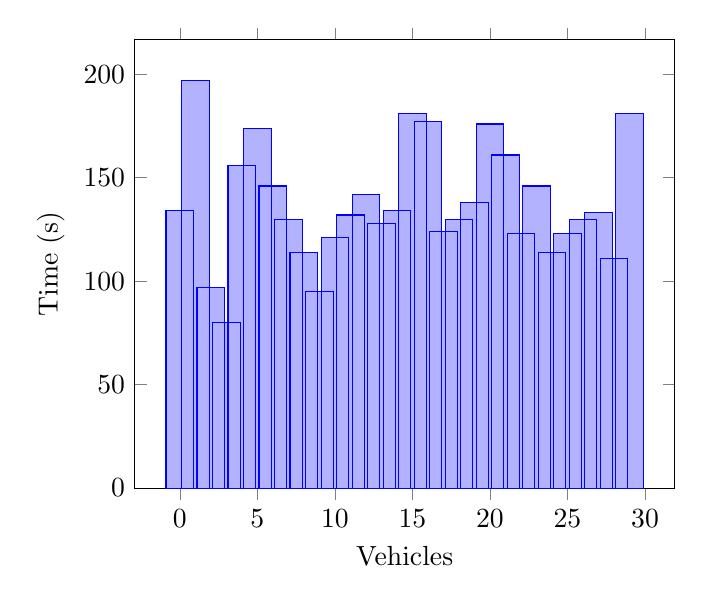
\begin{tikzpicture}
\begin{axis}[
legend style={anchor=west},
xlabel=Vehicles,
ylabel=Time (s),
ymin=0,
ybar,
]
\addplot coordinates {
(0, 134)
(1, 197)
(2, 97)
(3, 80)
(4, 156)
(5, 174)
(6, 146)
(7, 130)
(8, 114)
(9, 95)
(10, 121)
(11, 132)
(12, 142)
(13, 128)
(14, 134)
(15, 181)
(16, 177)
(17, 124)
(18, 130)
(19, 138)
(20, 176)
(21, 161)
(22, 123)
(23, 146)
(24, 114)
(25, 123)
(26, 130)
(27, 133)
(28, 111)
(29, 181)
};

\end{axis}
\end{tikzpicture}
\label{tik:100:96}
\caption{100 percent diving with GSC on route $96$}
\end{figure}
